%\documentclass[a4paper,10pt]{jarticle}
%\documentclass[]{jarticle}
\documentclass[10pt]{jarticle}
\usepackage[dvipdfmx]{graphicx}
\usepackage{ascmac}
\usepackage{here}
\usepackage{txfonts}
\usepackage{listings, jlisting}
\renewcommand{\lstlistingname}{Listing}
\lstset{
  language=c,
  basicstyle=\ttfamily\scriptsize,
  commentstyle=\textit,
  classoffset=1,
  keywordstyle=\bfseries,
  frame=tRBl,
  framesep=5pt,
  showstringspaces=false,
  numbers=left,
  stepnumber=1,
  numberstyle=\tiny,
  tabsize=2
}

%本文領域を広め(空白箇所マージン領域を小さめ)に設定
\setlength{\textwidth}{179mm}
\setlength{\textheight}{251mm}
\setlength{\topmargin}{-2cm}
\setlength{\oddsidemargin}{-1cm}
\setlength{\evensidemargin}{-1cm}

\begin{document}
\begin{titlepage}
\begin{center}
\vspace*{200truept}
{\Huge\bf プログラミング I}\\ % タイトル
\vspace*{10truept}
\hspace*{200truept}
{\Large Report\#1}\\ % サブタイトル(なければコメントアウト)
\vspace*{320truept}
\end{center}
\begin{flushleft}
{\Large
  \hspace*{300truept}
  提出日 :2012年6月14日(木)\\
  \hspace*{300truept}
  所 属 :工学部情報工学科\\
  \hspace*{300truept}
  学籍番号:128569G\\
  \hspace*{300truept}
  氏 名 :當眞 大千\\
}
\end{flushleft}
\end{titlepage}

\pagenumbering{roman}
\tableofcontents
\newpage
\pagenumbering{arabic}
\section{新規にtrupperプログラムを作成せよ}
標準ライブラリ関数 islower(), toupper()を使い、下記のtrlowupプログラムを書き換えて、新規にtrupperプログラムを作成せよ。
\subsection{サンプルプログラム}
\subsubsection{ソースコード}
\lstinputlisting[caption=trlowup.c,label=trlowup]
{./prog/trlowup.c}

\subsubsection{実行結果}
\lstinputlisting[caption=Result,label=trlowup-result]
{./result/trlowup}

% 改行するには\\を入れる
% 新しい段落は2回改行する
〜〜ということが分かる!
すごい。やったね!\\

Listing \ref{trlowup}はプログラムです。

Listing \ref{trlowup-result}は実行結果です。

% 囲むと枠付きになる
\begin{itembox}[l]{オイラーの公式}
  オイラーの公式($e^{i\theta}=\cos\theta+i\sin\theta$)は,とても不思議
  な式である.もともと,幾何学的な意味を持つ三角関数と,解析的な指数関数が,
  虚数を介して,とても単純な関係にあることを示している.
\end{itembox}

\begin{boxnote}
  さむーい
\end{boxnote}

% newpageで新しいページになる
\newpage
\section{問題2}
これは問題2である。
\subsection{エアコン}
エアコンは文明の利器
\subsubsection{寒い}
だけど寒い

\newpage
\section{殺伐とした…}
\begin{figure}[h]
  \begin{center}
    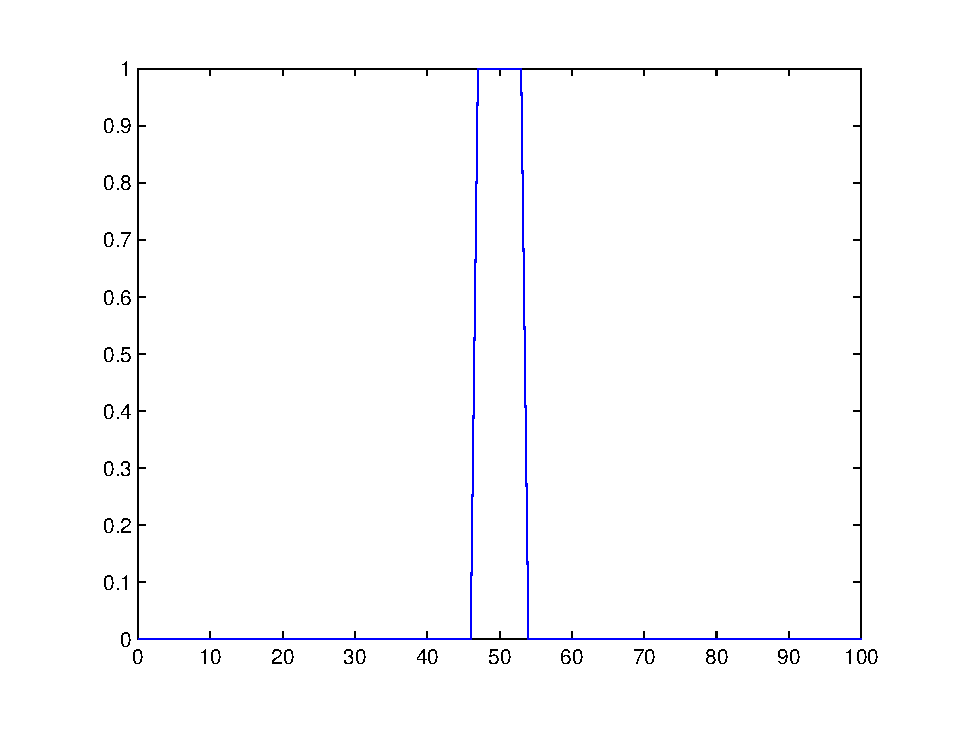
\includegraphics[width=13cm]{pic/problem4.eps}
  \end{center}
\end{figure}

\section{数式}
数式も余裕
\[
\mu_A (x) =
\left\{
  \begin{array}{lll}
    0             & (x \leq 8)\\
    \frac{1}{10}x - \frac{8}{10}  & (8 \leq x \leq 18)\\
   -\frac{1}{14}x + \frac{32}{14} & (18 \leq x \leq 32)\\
  \end{array}
\right.
\]
\[
\mu_B (x) =
\left\{
  \begin{array}{llll}
    0             & (x \leq -3)\\
    \frac{1}{9}x + \frac{1}{3}  & (-3 \leq x \leq 6)\\
   -\frac{1}{18}x + \frac{4}{3} & (6 \leq x \leq 24)\\
    0             & (x \geq 24)\\
  \end{array}
\right.
\]

\section{参考文献の参照のやり方}
\cite{google} で検索したら全て分かりました!

\begin{thebibliography}{99}
  \bibitem{google}%何か目印となる単語をいれておく
    Google\\
    \verb|http://www.google.co.jp|
\end{thebibliography}

\end{document}

